\documentclass[11pt,letterpaper]{article}

\usepackage{graphicx}

\usepackage{multicol}
\usepackage[top=20mm,bottom=20mm,left=15mm,right=15mm]{geometry}

\usepackage[font={small,sf}]{caption}
\captionsetup[figure]{labelfont=bf}
\captionsetup[table]{labelfont=bf}


\usepackage{sidecap}
\sidecaptionvpos{figure}{c}


% define new environments
\usepackage{amsthm}
\theoremstyle{definition}
\newtheorem*{hypothesis}{Hypothesis}
\newtheorem*{objective}{Objective}

% per-section figure numbering
\usepackage{chngcntr}
\counterwithin{figure}{section}
% use arabic section numbering for figures
\renewcommand{\thefigure}{\arabic{section}.\arabic{figure}}

% use roman number formatting for sections
\renewcommand\thesection{\Roman{section}}

% disable subsection numbering
\setcounter{secnumdepth}{1}

\usepackage[super,sort&compress]{natbib}

% define multiple reference lists
\usepackage{multibib}
\newcites{self,own,ref}{Refereed publications in thesis,Other refereed publications,References}


% emphasize author name
\newcommand{\emphname}[1]{\underline{\textbf{#1}}}

% emphasize label
\newcommand{\emphlab}[1]{\textbf{\textsf{#1}}}

% cite figure and table
\newcommand{\citefig}[1]{\emphlab{Figure~\ref{fig:#1}}}
\newcommand{\citetable}[1]{\emphlab{Table~\ref{tbl:#1}}}

\begin{document}

\begin{titlepage}

\setlength{\topmargin}{30mm}

\begin{center}
 
\textsc{\Large Committee meeting report}\bigskip

{\huge \bfseries Clinical genomics of medulloblastoma molecular subgroups}\\[10mm]

\begin{minipage}{0.6\textwidth}
\begin{multicols}{2}
	\begin{flushleft}
		\large \emph{Student:}\\
		David J. H. \textsc{Shih}
	\end{flushleft}
	\vfill
	\columnbreak
	\begin{flushright}
		\large \emph{Supervisors:}\\
		Dr.~Michael D. \textsc{Taylor}\\
		Dr.~Gary \textsc{Bader}\\
	\end{flushright}
	\begin{flushright}
		\large \emph{Committee:}\\
		Dr.~Meredith \textsc{Irwin}\\
		Dr.~Quaid \textsc{Morris}
	\end{flushright}
\end{multicols}
\end{minipage}

\vspace{20mm}

{ \large 
\textbf{Janurary 21, 2014}\\
\medskip
Peter Gilgan Centre for Research and Learning\\
686 Bay St\\
13th floor, Room 13.9701
}

\vspace{40mm}

\begin{flushleft}
	{ \large
	\textbf{Start date:} Janurary 3, 2011\\
	\textbf{Last meeting date:} April 24, 2012\\
	\medskip
	\textbf{Course requirements:} Complete\\
	\medskip
	\textbf{Refereed publications in thesis:} 3\\
	\textbf{Other refereed publications during program:} 13\\
	\textbf{Total refereed publications during program:} 16\\
	}
\end{flushleft}


\end{center}

\end{titlepage}


\clearpage

\bibliographystyleself{nature}
\bibliographyself{self}
\bigskip
$^*$ These authors contributed equally.

\clearpage

\bibliographystyleown{nature}
\bibliographyown{shih}

\clearpage

\section*{Summary of progress}

\nociteself{shih14,shih12,northcott12}

All aims have been completed.

\begin{description}
	\item[Aim I] Molecular classification of medulloblastoma in clinical contexts: \textbf{published} \citeself{northcott12}
	\item[Aim II] Target identification by copy-number profiling of medulloblastoma: \textbf{published} \citeself{shih12}
	\item[Aim III] Clinical prognostication within medulloblastoma subgroups: \textbf{in press} \citeself{shih14}
\end{description}

\nociteown{ramaswamy13,remke13,dey13,markant13,natarajan13,zhukova13,dubuc13,diaz12,jones12,wu12,rausch12,dubuc12,northcott11}

\listoffigures

\clearpage


\section*{Overview}

Medulloblastoma is the most common solid childhood malignancy \citeref{mainprize00}. Current therapy for medulloblastoma --- including surgical resection, radiation of the entire brain and spinal cord, and aggressive chemotherapy --- yields five-year survival rates of 60-70\% \citeref{gajjar06}. Survivors are often left with significant neurological, intellectual, and physical disabilities secondary to the effects of these non-specific, cytotoxic therapies on the developing nervous system \citeref{spiegler04,mabbott05}.

Recent evidence suggests that medulloblastoma in fact comprises a group of biologically distinct molecular entities whose clinical and genetic differences may require separate therapeutic strategies \citeref{thompson06,kool08,northcott11a,remke11,cho11}. Four principal subgroups\citeref{taylor12} of medulloblastoma have been identified: WNT, SHH, Group~3, and Group~4, and there is preliminary evidence for clinically significant subdivisions of the subgroups \citeref{northcott11a,cho11,remke11,taylor12,northcott11b}. Targeted therapies based on the genetics of the disease are not currently in use. However, inhibitors of the Sonic Hedgehog (Shh) pathway activator, Smoothened, have shown some early evidence of efficacy \citeref{rudin09}. With a deeper understanding of the genomics and biology of medulloblastoma subgroups, we hope to herald a new era of medulloblastoma treatment based on selective, specific, targeted therapy.

My study will focus on the following three obstacles that hinders the development of targeted therapy against medulloblastoma molecular subgroups:

\begin{enumerate}
	\item The lack of a clinically applicable assay for molecular subgrouping of medulloblastoma.
	\item The paucity of actionable targets for WNT, Group~3, and Group~4 medulloblastomas.
	\item Current clinical prognostication of medulloblastoma does not consider molecular subgroups.
\end{enumerate}

The objectives of my study are to provide viable solutions to these issues and to demonstrate the clinical significance of molecular classification.


\subsection{Aim I: Molecular classification of medulloblastoma in clinical contexts}

Although the retrospective classification of medulloblastoma has been scientifically informative, molecular subgrouping has not been applied in the context of a prospective clinical trial. One major obstacle is the lack of fresh-frozen samples for most clinical cases. Expression profiling, on which molecular classification was based, depends on the availability of high-quality RNA. In contrast, clinical samples are routinely subjected to formalin-fixation and paraffin-embedding (FFPE), which preserves tissue integrity but causes nucleic acid degradation. To facilitate the development of therapy specifically targeted against molecular subgroups, we sought to establish an molecular subgrouping assay that can be clinically applied on FFPE samples. I have established an analytic pipeline to molecular subgrouping using expression data generated by nanoString assays, and demonstrated its high classification accuracy on FFPE samples \citeself{northcott12}. To further make the assay clinically applicable, I have implemented several quality-control measures that identify cases which cannot be reliably assigned molecular subgroup, due to poor specimen quality or assay reaction failure.

\subsection{Aim II: Target identification by copy-number profiling of medulloblastoma}

After having established a clinically applicable molecular classification methodology, I turned to the problem of identifying molecular targets in medulloblastoma. Unlike SHH medulloblastomas, actionable targets for WNT, Group~3, and Group~4 tumours have yet been identified. However, prior attempts may have been underpowered to discriminate the genomic differences among the four molecular subgroups. To this end, the Medulloblastoma Advanced Genomics International Consortium (MAGIC), consisting of scientists and physicians from 43 cities across the globe, has gathered $>1200$ medulloblastomas. Paul Northcott and I have analyzed the genomic copy-number profiles of the tumours by Single Nucleotide Polymorphism (SNP) arrays. We have identified genes and pathways that characterize each medulloblastoma subgroup \citeself{shih12}.

\subsection{Aim III: Clinical prognostication within medulloblastoma subgroups}

Prior clinical prognostication studies in medulloblastoma have identified biomarkers without discriminating between the molecular subgroups of medulloblastoma. Given that medulloblastoma subgroups are biologically and molecular distinct disease entities, we hypothesized incorporating molecular subgroup into prognostication can enhance the accuracy of survival prediction and improve the reliability of risk stratification. Practical and reliable identification of risk could allow for therapy intensification in high-risk children to improve survival and therapy de-escalation in low-risk children to avoid complications of therapy. By identifying clinical and molecular biomarkers within medulloblastoma subgroups, I have designed risk stratification schemes for SHH, Group~3, and Group~4 medulloblastoma that can achieve unpredented levels of prognostication accuracy.


\clearpage


\section{Molecular classification of medulloblastoma in clinical contexts}

\begin{objective}
To develop a clinically applicable assay for molecular classification of medulloblastoma.
\end{objective}

The nanoString nCounter technology \citeref{geiss08} was used to directly measure the expression level of 22 medulloblastoma subgroup specific signature genes. The nanoString assay directly interrogates nucleic acid levels without polymerase chain reaction (PCR) amplification (or other enzymatic reactions) in multiplexed system, using pairs of fluorescent probes that bind to target sequences. We developed an analytic method that can accurately predict molecular subgroups of medulloblastoma, even on archival FFPE samples \citeself{northcott12}.

A set of widely used classifiers (e.g. support-vector machine, linear discriminant analysis, multinomial logistic regression, k-nearest neighbour, pattern analsis of microarrays) were trained using a training set of 101 medulloblastomas with known subgroup affiliations. The classifiers were tuned and assessed using cross-validation. The most accurate classifier (across all tested accuracy measures) was selected for classification.

\begin{figure}[hb]
	\begin{center}
		\includegraphics[width=\textwidth]{fig/nanostr-class/nanostr-valid.pdf}
	\end{center}
	\caption[Validation of classification assay on independent medulloblastoma cohorts]
	{
	Validation of classification assay on independent medulloblastoma cohorts.
	\textbf{a-c}, Expression heatmaps of nanoString class-predicted medulloblastomas of known subgroup status as published by Remke et al.\citeref{remke11} (a), Cho et al.\citeref{cho11} (b), and Kool et al.\citeref{kool08} (c). Samples are sorted according to subgroup predictions. Known expression subgroup affiliations and erroneously classified cases are marked above the heatmap.
	\textbf{d}, \emph{Left}, Pie chart depicting the known subgroup distribution of medulloblastomas from the three independent cohorts analyzed in \textbf{a-c} ($n = 130$) and the subgroups predicted by nanoString profiling. Misclassified cases are marked within each slice according to the predicted subgroups. \emph{Right}, Pie chart of class prediction accuracy ($127/130$) from the validation set. Adapted from Northcott et al.\citeself{northcott12}
	}
	\label{fig:nanostr-valid}
\end{figure}

The assay was validated on an external set of 130 non-overlapping medulloblastomas, and it achieved an accuracy of 98\% (\citefig{nanostr-valid}). Further, the assay yielded reproducible predictions when repeated in three independent laboratories \citeself{northcott12}. The clinical applicability of the assay was demonstrated by its predictive accuracy on FFPE samples of archival ages $\leq 8$ years (\citefig{nanostr-ffpe}). The accuracy decreased on older FFPE samples, presumably due to poorer RNA integrity, though standard measurements of RNA quality were not correlated with accuracy \citeself{northcott12}.

\begin{figure}[ht]
	\begin{center}
		\includegraphics[width=\textwidth]{fig/nanostr-class/nanostr-ffpe.pdf}
	\end{center}
	\caption[Classification performance on formalin-fixed paraffin embedded archival samples]
	{
	Classification performance on formalin-fixed paraffin embedded archival samples.
	\textbf{a}, Class prediction accuracy in relation to sample age of archival medulloblastomas stored as FFPE material ($n = 84$). Samples obtained within the past 8 years exhibit accuracies of $\geq 95\%$, as demarcated by the red vertical line.
	\textbf{b}, Heatmap of nanoString data showing class predictions for FFPE cases of $\leq 8$ years confidently predicted by the assay ($n = 28$). Samples are sorted according to subgroup prediction. All cases satisfying prediction probability threshold were assigned to the correct subgroup ($28/28$). Adapted from Northcott et al.\citeself{northcott12}
	}
	\label{fig:nanostr-ffpe}
\end{figure}

Since the initial publication of the assay for molecular classification, we have analyzed over 1000 medulloblastoma samples and identified a few cases were replicate assays yielded conflicting results. Further examination revealed that poor sample quality and suboptimal assay conditions likely contributed to classification discrepancies. Therefore, additional quality control measures were implemented, which are especially important for developing this assay further for Clinical Laboratory Improvement Amendments (CLIA) certification.

Given that standard measurements of RNA quality were insufficient for predicting assay accuracy \citeself{northcott12}, the mean signals of the endogenous control probes included in the nanoString assay were used to assess whether sufficient quantities of intact, undegraded were present in the samples, using a outlier detection method. A Gaussian mixture model was fitted to all collected nanoString data to establish the nominal range for mean endogenous-control signals. Samples with mean signals that deviate significantly from this range at a significance level of 0.01 were identified as outliers. Such samples, due to extensive RNA degradation, cannot be assigned a molecular subgroup, and they may require classification using DNA copy-number or methylation profiling.

Samples with sufficiently high-quality RNA may yet yield uninterpretable results when suboptimal assay conditions confound the measurements. Therefore, signals from positive control and negative control probes are examined to identify assay reactions that may have failed and hence produced unreliable measurements. The current collection of nanoString data was used to establishe the nominal range of positive and negative signals, using Gaussian mixture and multiple negative binomial models, respectively. As above, measurements that deviate significantly from the nominal range at a significance level of 0.01 were considered outliers. Samples that fail this quality control criterion may simply be run again.

Furthermore, multi-sample assays are not amendable to reproducible clinical analysis of samples in real-time, owing to time constraints and potential batch effects. Single-sample nanoString assays were therefore tested for concordance with previous results. With the appropriate quality control and improved normalization procedures implemented, 100\% concordance was achieved with single-sample assays, which further enhanced the clinical utility of molecular classification assay.

Above all, a rapid, reliable, and reproducible assay was developed for assigning molecular subgroups to clinical samples, available as frozen or recent FFPE material, and this assay has been developed further use in a clinical laboratory. Critically, stringent quality control must accompany the nanoString classification assay, lest its potentials be shadowed by concerns of reproducibility and predictability, an ignominy that has long plagued the microarray technology \citeref{shi08,deronde10,weigelt10,ein-dor06,frantz05,michiels05,ioannidis05,marshall04,check04,tan03,tilstone03}.


\clearpage


\section{Target identification by copy-number profiling of medulloblastoma}

\begin{hypothesis}
Each medulloblastoma molecular subgroup is characterized by specific genomic aberrations.
\end{hypothesis}

Copy-number profiles were generated on $> 1200$ medulloblastomas using the Affymetrix Genome-wide SNP6 platform. After quality control and clinical criteria filtering, copy-number profiles of $1087$ primary medulloblastomas were available for further analysis in identifying somatic copy-number aberrations (SCNAs): regions of aberrant gains and losses in the tumour genome. The tumours were stratified based on molecular subgroups, as determined by the method described in \textbf{Aim I}. The copy-number and cytogenetic profiles of medulloblastoma subgroups were highly divergent, demonstrating that medulloblastoma subgroups are genomically heterogeneous (\citefig{cn-heatmap}--\citefig{broad-events}). Indeed, when the cohort was analyzed by each subgroup independently, an increased number of SCNAs were identified, many of which were subgroup-enriched (\citefig{subgroup-specificity}).

\begin{SCfigure}[5][t]
	\centering
	\includegraphics[width=0.3\textwidth]{fig/magic-cn/cn-heatmap.png}
	\caption[Genome-wide copy-number profile of medulloblastoma subgroups]
	{
	Genome-wide copy-number profile of medulloblastoma subgroups.
	Copy-number profiling was performed on 1087 non-overlapping primary medulloblastomas. Shown is a copy number heatmap for 827 cases classified according to medulloblastoma subgroup based on matched gene expression data.  Amplifications are shown in red and deletions in blue.
	}
	\label{fig:cn-heatmap}
\end{SCfigure}

\begin{SCfigure}[5][b]
	\centering
	\includegraphics[width=0.4\textwidth]{fig/magic-cn/broad-events.pdf}
	\caption[Frequency and significance of broad cytogenetic events]
	{
	Frequency and significance of broad cytogenetic events across medulloblastoma subgroups.
	Gains are plotted in red and deletions in blue, shaded according to significance ($q < 0.1$, binomial test).
	}
	\label{fig:broad-events}
\end{SCfigure} 

Among the recurrent high-level amplifications (copy-number $\geq 5$) identified (\citefig{high-level-amps}), the most prevalent events targeted members of the MYC family (\emph{MYCN}, \emph{MYC}, \emph{MYCL1}), with \emph{MYCN} predominantly amplified in SHH and Group~4, \emph{MYC} in Group~3, and \emph{MYCL1} in SHH medulloblastomas.
The most common homozygous deletions targeted known tumour suppressors \emph{PTEN}, \emph{PTCH1}, and \emph{CDKN2A/B}, all of which were enriched in SHH tumours (\citefig{homo-del}). A selected set of genes were assessed using custom nanoString assays, and 90.9\% of events were verified (\citefig{nanostr-verification}). Additional genes were validated on external cohorts by interphase fluorescence \emph{in situ} hybridization (\citefig{mdm4-fish}, \citefig{acvr2b-fish}).

The disparate genomic landscapes of medulloblastoma subgroups lead to the identification of a multitude of focal SCNAs that characterize each molecular subgroup (\citefig{shh-gistic}, \citefig{group3-gistic}, \citefig{group4-gistic}). Novel genes identified in this study include: \emph{PPM1D}, \emph{PIK3C2B}, and \emph{MDM4} in SHH (\citefig{shh-amps-igv}); \emph{ACVR2A}, \emph{ACVR2B}, and \emph{TGFBR1} in Group~3 (\citefig{group3-amps-igv}); and \emph{NFKBIA} and \emph{USP4} in Group~4 (\citefig{group4-dels-igv}). Conversely, WNT medulloblastoma have few recurrent SCNAs (\citefig{genome-coverage}). 

SHH medulloblastoma, which is characterized by activation of Shh signaling \citeref{northcott11a,remke11,cho11,kool08,taylor12}, exhibit frequent SCNAs in the Shh pathway. Genes involved in focal SCNAs amplifications are significantly associated with SHH medulloblastoma signatures genes (\citefig{shh-signature}), suggesting that copy-number changes contribute in part to the altered expression signatures previously observed in SHH tumours. Accordingly, positive regulators of Shh signaling (\emph{MYCN} and \emph{GLI2}) were recurrently amplified, while a negative regulator of Shh signaling (\emph{PTCH1}) was recurrently lost. Consistent with their functions in the same pathway, these events were mutually exclusive; however, they lead to different clinical outcomes (\citefig{shh-me}). In additional to Shh signaling, other core pathways recurrently disrupted in SHH medulloblastoma are TP53 signaling and RTK/PI3K signaling (\citefig{shh-pathways}).

The signaling pathways involved in Group~3 and Group~4 medulloblastomas are less well understood, as suggested by their names. Nonetheless, at the copy-number level, distinct pathways were dysregulated in Group~3 and Group~4 (\citefig{group3-vs-group4}). Group~3 tumours are characterized by amplification of \emph{MYC} and \emph{OTX2}, which occur in a mutually exclusive pattern (\citefig{group3-me}). This observation is consistent with the tendency of the two oncogenic transcription factors to bind the same promoter regions \citeref{bunt11}. Further, the TGF$\beta$ signaling pathway is frequently disrupted by SCNAs in Group~3. Conversely, the NF-$\kappa$B pathway appear to genetically targeted in Group 4 medulloblastomas.

While \emph{MYC} amplification is a known pivotal player Group~3, our data indicated that others genes in close proximity to the \emph{MYC} locus may also play cooperative roles. This locus was frequently disrupted by a multitude of high-level amplicons (\citefig{chromothr_myc}) as well as massively genomic rearrangements (\citefig{chromothr_myc_wgs}). These genomic aberrations are reminiscent of chromothripsis (chromosome shattering), which has recently been implicated in cancer formation \citeref{stephens11,liu11,kloosterman11b,magrangeas11,crasta12,molenaar12}, as well as in medulloblastoma \citeself{rausch12}. As a consequence of these events, the adjacent \emph{PVT1} gene and miR-1204 are frequently co-amplified with \emph{MYC}. Moreover, amplifications of the \emph{MYC}/\emph{PVT1} locus frequently result in the formation of fusion transcripts. Concurrent with MYC-PTV1 fusion expression, miR-1204 (hosted in PTV1) is upregulated (\citefig{myc-fusion_mir-expr}). \emph{MYC}, \emph{PVT1}, and miR-1204 all have been previously shown to play independent functional roles in other tumours \citeref{guan07,carramusa07,huppi08,barsotti12}, and may synergistically promote tumourigenesis.

The most prevalent focal gain (and previously neglected) in Group~4 was the somatic tandem duplication of the \emph{SNCAIP} gene (\citefig{sncaip-gain}). SNCAIP expression is highly elevated in Group~4 medulloblastomas (\citefig{sncaip-expr}). In fact, \emph{SNCAIP} duplication is further restricted to the Group~4$\alpha$ and may play a functional role in this medulloblastoma subtype (\citefig{group4-alpha-beta}). Another lab member, Vijay Ramaswamy, has begun functional characterization of this gene.

In summary, medulloblastoma subgroups are characterized by distinct genomic aberrations that dysregulated disparate signaling pathways. Importantly, the amplified genes and activated pathways identified in this study could serve as potential targets for therapeutic development in medulloblastoma subgroups.

\begin{SCfigure}[5]
	\centering
	\includegraphics[width=0.25\textwidth]{fig/magic-cn/subgroup-specificity.pdf}
	\caption[Significant regions of focal SCNA identified by GISTIC2]
	{
	Significant regions of focal SCNA identified by GISTIC2 in pan-cohort or subgroup-stratified analyses.
	A total of 62 significant regions were identified when the cohort was analyzed as a single group, whereas 110 significant regions were captured when the cohort was analyzed according to subgroup. The number of significant subgroup-enriched regions identified more than doubled (73 vs. 30) when the subgroups were analyzed independently.
	}
	\label{fig:subgroup-specificity}
\end{SCfigure}


\clearpage

\begin{SCfigure}[5]
	\centering
	\includegraphics[width=0.4\textwidth]{fig/magic-cn/high-level-amps.pdf}
	\caption[Recurrent high-level amplifications in medulloblastoma]
	{
	Recurrent high-level amplifications in medulloblastoma.
	Frequency of genes amplified (segmented copy-number $\geq 5$) in at least two samples are shown with the distribution of the event across subgroups. The number of genes mapping to the peak region as defined by GISTIC2 (where applicable) are listed in parentheses after the candidate driver gene.
	}
	\label{fig:high-level-amps}
\end{SCfigure}

\begin{SCfigure}[5]
	\centering
	\includegraphics[width=0.4\textwidth]{fig/magic-cn/homo-del.pdf}
	\caption[Recurrent homozygous deletions in medulloblastoma]
	{
	Recurrent homozygous deletions in medulloblastoma.
	Frequency of genes targeted by homozygous deletion (segmented copy-number $\leq 0.7$) in at least two samples are shown.
	}
	\label{fig:homo-del}
\end{SCfigure}

\begin{SCfigure}[5]
	\centering
	\includegraphics[width=0.3\textwidth]{fig/magic-cn/nanostr-verification.pdf}
	\caption[Verification of focal SCNAs by nanoString]
	{
	Verification of focal SCNAs by nanoString.
	Genes inferred to be focally amplified by SNP6 were interrogated using a custom nanoString CodeSet across a set of 192 medulloblastomas selected from our cohort. Bar-plot shows the number of samples for which each gene is verified (red) or not (black). An overall verification rate of 90.9\% was achieved.
	}
	\label{fig:nanostr-verification}
\end{SCfigure}

\clearpage

\begin{figure}[h]
	\begin{center}
		\includegraphics[width=\textwidth]{fig/magic-cn/shh-gistic.pdf}
	\end{center}
	\caption[Landscape of SCNAs in SHH medulloblastoma]
	{
	Landscape of SCNAs in SHH medulloblastoma.
	GISTIC2 significance plot of amplifications (red) and deletions (blue) observed in the SHH subgroup is shown.
	Labeled cytobands indicate significant regions that satisfied multiple criteria to qualify as a potential somatic event. The number of genes mapping to each significant region are shown in parentheses next to the cytoband label.  Regions over-represented in SHH are highlighted in red.
	}
	\label{fig:shh-gistic}
\end{figure}

\clearpage

\begin{SCfigure}
	\centering
	\includegraphics[width=0.7\textwidth]{fig/magic-cn/shh-amps-igv.pdf}
	\caption[Recurrent amplifications of \emph{PPMID}, \emph{MDM4}, and \emph{PIK3C2B} in SHH medulloblastoma]
	{
	Recurrent high-level amplifications of \emph{PPMID} and co-amplification of \emph{MDM4} and \emph{PIK3C2B} in SHH medulloblastoma.
	Segmented copy-number tracks are shown for the amplified loci (17q23 and 1q23).
	}
	\label{fig:shh-amps-igv}
\end{SCfigure}

\begin{SCfigure}
	\centering
	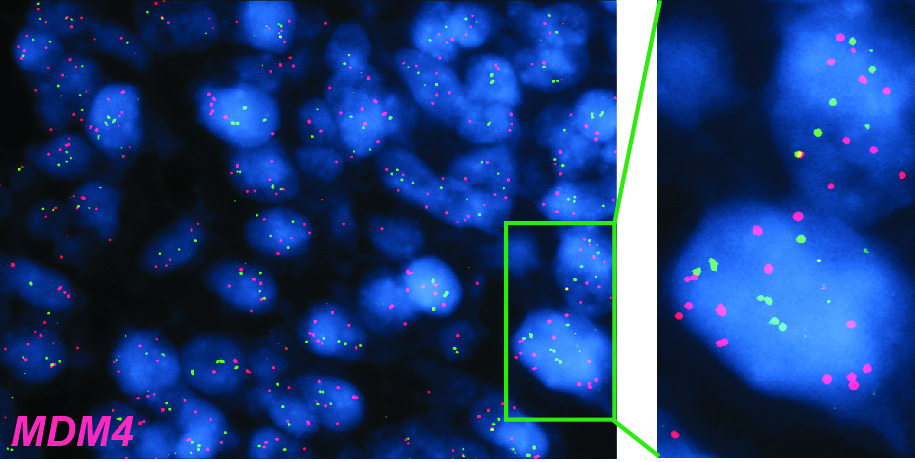
\includegraphics[width=0.4\textwidth]{fig/magic-cn/mdm4-fish.jpg}
	\caption[Validation of \emph{MDM4} amplification in medulloblastoma]
	{
	Validation of \emph{MDM4} amplification in medulloblastoma.
	Interphase fluorescence \emph{in situ} hybridization (FISH) of the \emph{MDM4} locus confirmed amplification in 8.2\% (12/146) of external cases present on a medulloblastoma tissue microarray (work by Andrey Korshunov).
	}
	\label{fig:mdm4-fish}
\end{SCfigure}

\clearpage

\begin{figure}[h]
	\begin{center}
		\includegraphics[width=\textwidth]{fig/magic-cn/group3-gistic.pdf}
	\end{center}
	\caption[Landscape of SCNAs in Group~3 medulloblastoma]
	{
	Landscape of SCNAs in Group~3 medulloblastoma.
	GISTIC2 significance plot of recurrent amplifications and deletions in Group~3 is shown. Events highlighted in yellow are enriched in Group~3.
	}
	\label{fig:group3-gistic}
\end{figure}

\clearpage

\begin{SCfigure}
	\centering
	\includegraphics[width=0.7\textwidth]{fig/magic-cn/group3-amps-igv.pdf}
	\caption[Recurrent amplifications target receptors of the TGF$\beta$ superfamily in Group~3]
	{
	Recurrent amplifications target receptors of the TGF$\beta$ superfamily in Group~3.
	Segmented copy-number tracks of Group~3 medulloblastomas show recurrent high-level amplifications affecting \emph{ACVR2A} (2q22), \emph{ACVR2B} (3p22), and \emph{TGFBR1} (9q22).
	}
	\label{fig:group3-amps-igv}
\end{SCfigure}

\begin{SCfigure}[3.0]
	\centering
	\includegraphics[width=0.3\textwidth]{fig/magic-cn/acvr2b-fish.jpg}
	\caption[Validation of \emph{ACVR2B} amplification]
	{
	Validation of \emph{ACVR2B} amplification.
	FISH of the \emph{ACVR2B} locus confirmed presence of amplification in an external cohort of medulloblastomas on a TMA (work by Andrey Korshunov).
	}
	\label{fig:acvr2b-fish}
\end{SCfigure}

\clearpage

\begin{figure}[h]
	\begin{center}
		\includegraphics[width=\textwidth]{fig/magic-cn/group4-gistic.pdf}
	\end{center}
	\caption[Landscape of SCNAs in Group~4 medulloblastoma]
	{
	Landscape of SCNAs in Group~4 medulloblastoma.
	GISTIC2 significance plot of amplification and deletion regions in Group~4 is shown. Events highlighted in green are enriched in Group~4.
	}
	\label{fig:group4-gistic}
\end{figure}

\clearpage

\begin{SCfigure}[2.0]
	\centering
	\includegraphics[width=0.3\textwidth]{fig/magic-cn/group4-dels-igv.pdf}
	\caption[NF-$\kappa$B pathway is recurrently targeted in Group~4]
	{
	NF-$\kappa$B pathway is recurrently targeted in Group~4.
	Recurrent focal deletions disrupt \emph{NFKBIA} and \emph{USP4}, negative regulators of the NF-$\kappa$B pathway, in Group~4 medulloblastoma.
	}
	\label{fig:group4-dels-igv}
\end{SCfigure}

\begin{SCfigure}[5]
	\centering
	\includegraphics[width=0.3\textwidth]{fig/magic-cn/genome-coverage}
	\caption[WNT medulloblastomas sustain a paucity of recurrent focal SCNAs.]
	{
	WNT medulloblastomas sustain a paucity of recurrent focal SCNAs.
	Bar-plots of the proportion of genome recurrently disrupted by focal SCNAs are depicted for each medulloblastoma subgroup.
	}
	\label{fig:genome-coverage}
\end{SCfigure}

\clearpage

\begin{figure}
	\centering
	\includegraphics[width=0.8\textwidth]{fig/magic-cn/shh-me.pdf}
	\caption[Mutually exclusivity and clinical significance of focal SCNAs in SHH medulloblastomas]
	{
	Mutually exclusivity and clinical significance of focal SCNAs in SHH medulloblastomas.
	Mutual exclusivity analysis of focal SCNAs in SHH medulloblastoma reveals that the most prevalent events in this subgroup do not co-occur in the same sample and collectively contribute to 23\% of cases, suggesting functional redundancy of SCNAs. Nevertheless, the mutually exclusive events exhibit distinct clinical outcome. Patients exhibiting either \emph{MYCN} or \emph{GLI2} amplification have poor clinical outcomes, while those exhibiting focal \emph{PTCH1} deletion have improved overall survival.
	}
	\label{fig:shh-me}
\end{figure}

\begin{SCfigure}[5]
	\centering
	\includegraphics[width=0.3\textwidth]{fig/magic-cn/shh-signature.pdf}
	\caption[Overlap between SHH signature genes and genes targeted by focal SCNAs in SHH]
	{
	Significant overlap between SHH signature genes and genes targeted by focal SCNAs in SHH.
	Bar-plots show the overlap significance based on permutation tests between SHH signature genes reported in the Cho (\emph{left}) or Northcott (\emph{right}) studies and genes mapping to focal SCNAs in our dataset. Dashed line indicates significance threshold ($\alpha = 0.05$).
	}
	\label{fig:shh-signature}
\end{SCfigure}

\clearpage

\begin{figure}[h]
	\begin{center}
		\includegraphics[width=0.8\textwidth]{fig/magic-cn/shh-pathways.pdf}
	\end{center}
	\caption[Core pathways genetically targeted in SHH medulloblastoma]
	{
	Core pathways genetically targeted in SHH medulloblastoma.
	Summary of SCNAs affecting components of Shh signaling, TP53 signaling, and RTK/PI3K signaling are depicted. Colours reflect the frequency by which the respective genes are targeted by focal or broad events in SHH medulloblastomas (red for amplification, blue for deletion). Significance values indicate the prevalence with which each pathway is targeted in SHH vs. non-SHH cases (Fisher's exact test).
	}
	\label{fig:shh-pathways}
\end{figure}

\clearpage

\begin{figure}[h]
	\begin{center}
		\includegraphics[width=0.7\textwidth]{fig/magic-cn/group3-me.pdf}
	\end{center}
	\caption[Mutual exclusivity of \emph{MYC}, \emph{OTX2}, and \emph{DDX31} aberrations in Group~3]
	{
	Mutual exclusivity of \emph{MYC}, \emph{OTX2}, and \emph{DDX31} aberrations in Group~3.
	Analysis of focal SCNAs reveals that \emph{MYC} amplification and \emph{OTX2} amplification are completely mutually exclusivity, and these events are prognostic significant: \emph{MYC} amplified cases show poorer overall survival.
	}
	\label{fig:group3-me}
\end{figure}

\begin{SCfigure}
	\centering
	\includegraphics[width=0.4\textwidth]{fig/magic-cn/group3-pathways.pdf}
	\caption[TGF$\beta$ signaling is recurrently disrupted by SCNAs in Group~3]
	{
	TGF$\beta$ signaling is recurrently disrupted by SCNAs in Group~3.
	SCNAs affecting the TGF$\beta$ pathway comprise 20.2\% of Group~3 cases and are significantly enriched in Group~3 compared to non-Group~3 cases (Fisher's exact test).
	}
	\label{fig:group3-pathways}
\end{SCfigure}

\begin{SCfigure}
	\centering
	\includegraphics[width=0.5\textwidth]{fig/magic-cn/group3-vs-group4.pdf}
	\caption[Aberrations disrupt distinct pathways in Group~3 and Group~4 medulloblastomas]
	{
	Aberrations disrupt distinct pathways in Group~3 and Group~4 medulloblastomas.
	Enrichment plot of gene sets disrupted by SCNAs in Group~3 vs. Group~4 medulloblastomas.
	}
	\label{fig:group3-vs-group4}
\end{SCfigure}

\clearpage

\begin{figure}[h]
	\begin{center}
		\includegraphics[width=0.9\textwidth]{fig/magic-cn/sncaip-gain.png}
	\end{center}
	\caption[Focal gains recurrently target \emph{SNCAIP} in Group~4]
	{
	Focal gains recurrently target \emph{SNCAIP} in Group~4.
	\emph{Left}, Segmented copy-number tracks of 317 Group~4 tumours shows a highly recurrent region of focal gain at 5q23.2 targeting a single gene: \emph{SNCAIP}, observed in 10.4\% of Group~4 cases (33/137). Whole-genome sequencing confirms that \emph{SNCAIP} is tandemly duplicated\citeself{shih12}. \emph{Right}, Analysis of matched-germline confirms that \emph{SNCAIP} duplication is somatic.
	}
	\label{fig:sncaip-gain}
\end{figure}

\begin{figure}[h]
	\begin{center}
		\includegraphics[width=0.9\textwidth]{fig/magic-cn/sncaip-expr.pdf}
	\end{center}
	\caption[\emph{SNCAIP} is a Group~4 signature gene]
	{
	\emph{SNCAIP} is a Group~4 signature gene.
	\emph{Left}, Box-plot depicting SNCAIP significant upregulation in Group~4 (Mann-Whitney test), as determined by expression analysis of a previously published cohort of 103 primary medulloblastoma \citeref{northcott11a}. SNCAIP ranks among the top 1\% of most highly expressed genes in Group~4 medulloblastoma (rank 39 out of 16758).
	\emph{Right}, Validation of SNCAIP as a Group~4 signature gene across five published medulloblastoma expression datasets: Thompson \citeref{thompson06}, Kool \citeref{kool08}, Fattet, Cho \citeref{cho11}, and Remke \citeref{remke11}. Expression datasets total 396 cases on four different array platforms. In all datasets, SNCAIP exhibited highest expression in Group~4.
	}
	\label{fig:sncaip-expr}
\end{figure}

\begin{figure}[h]
	\begin{center}
		\includegraphics[width=\textwidth]{fig/magic-cn/group4-alpha-beta.pdf}
	\end{center}
	\caption[\emph{SNCAIP} duplication is restricted to one subtype of Group~4]
	{
	\emph{SNCAIP} duplication is restricted to one subtype of Group~4.
	\textsf{a}, Non-negative matrix factorization (NMF) consensus clustering performed on expression profiles of Group~4 cases ($n = 188$) reveal two transcriptionally distinct subtypes of Group~4, designated $4\alpha$ and $4\beta$. SNCAIP duplicated is significantly enriched in the Group $4\alpha$ subtype (Fisher's exact test).
	\textsf{b}, SNCAIP expression is significantly elevated in Group $4\alpha$ compared to $4\beta$ (Mann-Whitney test).
	\textsf{c}, SNCAIP expression is copy number-driven in Group $4\alpha$. Group $4\alpha$ cases were stratified by \emph{SNCAIP} copy-number status. Samples harbouring SNCAIP duplication exhibit a significant \~1.5-fold increase in SNCAIP expression (Mann-Whitney test).
	}
	\label{fig:group4-alpha-beta}
\end{figure}

\begin{figure}[h]
	\begin{center}
		\includegraphics[width=\textwidth]{fig/magic-cn/chromothr_myc_ai.pdf}
	\end{center}
	\caption[A multitude of amplicons disrupt the \emph{MYC}/\emph{PVT1} locus]
	{
	A multitude of amplicons disrupt the \emph{MYC}/\emph{PVT1} locus.
	Copy-number plot of 8q24.21 is shown for a representative sample. Dots represent raw copy-number estimates and lines denote copy-number segments and state (red: gain, blue: loss). 71.4\% of \emph{MYC}-amplified (20/28) cases exhibit (partial) co-amplification of adjacent non-coding \emph{PVT1} gene and miR-1204. PVT1-MYC fusion transcripts were detected by RNA-seq, qRT-PCR, and Sanger sequencing in 8/20 samples \citeself{shih12}.
	}
	\label{fig:chromothr_myc}
\end{figure}

\begin{figure}[h]
	\begin{center}
		\includegraphics[width=0.7\textwidth]{fig/magic-cn/chromothr_myc_wgs.pdf}
	\end{center}
	\caption[Chromothripsis disrupts the \emph{MYC}/\emph{PVT1} locus.]
	{
	Chromothripsis disrupts the \emph{MYC}/\emph{PVT1} locus.
	Whole-genome sequencing confirms a complex pattern of rearrangements on 8q24 in a representative sample, reminiscent of chromothripsis (chromosome shattering).
	Plot shows chromosome 8 copy-number estimates (derived from read depth ratio of tumour vs. matched germline).
	Complex rearrangements are observed in concordance with a multitude of amplicons in the 8q24 region.
	}
	\label{fig:chromothr_myc_wgs}
\end{figure}

\begin{SCfigure}
	\centering
	\includegraphics[width=0.4\textwidth]{fig/magic-cn/chromothr-enrich.pdf}
	\caption[Chromothripsis frequently disrupt chr8 in Group~3 medulloblastoma]
	{
	Chromothripsis frequently disrupt chr8 in Group~3 medulloblastoma.
	Quantification of inferred chromothripsis across medulloblastoma subgroups reveal a significant enrichment of chromothripsis on chr8 in Group~3 ($q = 0.0004$, Fisher's exact test), as compared to the entire cohort. Samples exhibiting at least 10 copy-number state changes on a single chromosome were inferred to have undergone chromothripsis.
	}
	\label{fig:chromothr-enrich}
\end{SCfigure}

\begin{figure}[h]
	\begin{center}
		\includegraphics[width=0.5\textwidth]{fig/magic-cn/myc-fusion_mir-expr.pdf}
	\end{center}
	\caption[miR-1204 is upregulated in Group~3 cases harbouring PVT1-MYC fusions]
	{
	miR-1204 is upregulated in Group~3 cases harbouring PVT1-MYC fusions.
	Quantitative RT-PCR analysis of microRNAs hosted by PVT1 confirms upregulation of miR-1204 in Group~3 cases harbouring PVT1-MYC fusions (Mann-Whitney test). Samples were categorized as MYC-balanced/fusion(-) ($n = 4$), MYC-amplified/fusion(-) ($n = 6$), or MYC-amplified/fusion(+) ($n = 8$). Expression of microRNAs in MYC-balanced/fusion(-) samples served as baselines for determining relative expressions of the respective microRNAs in the other groups. Experiments were performed by John Peacock.
	}
	\label{fig:myc-fusion_mir-expr}
\end{figure}


\clearpage


\section{Clinical prognostication within medulloblastoma subgroups}

\begin{objective}
To stratify patients into risk groups based on clinical and molecular biomarkers within medulloblastoma subgroups.
\end{objective}

Current medulloblastoma protocols stratify patients based on clinical features: patient age, metastatic stage, extent of resection, and histological variant. The stark prognostic and genetic differences between the subgroups observed in \textbf{Aim II} suggest that subgroup-specific molecular biomarkers could improve patient prognostication.

\begin{SCfigure}[5][t]
	\includegraphics[width=0.3\textwidth]{fig/magic-clin/meta_cyto-markers.pdf}
	\caption[Sample sizes of recent prognostic marker studies]
	{
	Sample sizes of recent prognostic marker studies.
	This meta-analysis was performed by Marc Remke.
	}
	\label{fig:meta_cyto-markers}
\end{SCfigure}

To determine whether subgroup affiliation could support or supplant clinical variables for prognostication in medulloblastoma patients and to determine the effects of subgroup affiliation on cytogenetic biomarkers, we assembled an international discovery cohort of 673 medulloblastomas through MAGIC, for which we had both clinical follow-up and copy number data (Affymetrix SNP 6.0). To begin, I identified subgroup-specific copy-number aberrations (CNAs) and integrated them with clinical variables to develop subgroup-specific risk models based on the discovery cohort. In order to validate the models and ensure that the technique was generalizable to routine pathology laboratories, our colloborators (Andrey Korshunov and Stefan Pfister) then studied a panel of six cytogenetic biomarkers (\emph{GLI2}, \emph{MYC}, 11, 14, 17p, and 17q) using interphase fluorescent in-situ hybridization (FISH) on an FFPE medulloblastoma tissue microarray (TMA) that includes a set of 453 medulloblastomas that were treated at a single center and does not overlap with the discovery cohort.

The analysis of $> 1000$ medulloblastoma patients clearly demonstrates that subgroup affiliation enhances prognostication with clinical biomarkers, and that the majority of published molecular biomarkers are only relevant in the setting of a single subgroup. The combination of clinical variables, subgroup affiliation, and six cytogenetic markers analyzed on FFPE tissues can achieve an unprecedented level of prognostic prediction for medulloblastoma patients that is practical, reliable, and reproducible.

\begin{SCfigure}[5][b]
	\includegraphics[width=0.35\textwidth]{fig/magic-clin/surv_mb-subgroups.pdf}
	\caption[Overall survival curves for molecular subgroups of medulloblastoma]
	{
	Overall survival curves for molecular subgroups of medulloblastoma.
	Numbers below x-axis represent patients at risk of event; statistical significances are evaluated by log-rank tests; hazard ratio estimates (HR) are derived from Cox proportional-hazards analyses.
	}
	\label{fig:surv_mb-subgroups}
\end{SCfigure}

\clearpage

\subsection{Prognostic significance of clinical variables within medulloblastoma subgroups}

Many prior medulloblastoma biomarker publications were limited by sample size, a problem that will only be exacerbated once cohorts are divided into their molecular subgroups.  The current study includes 1126 medulloblastoma patients (673 discovery plus 453 validation patients), which is more than double the sample size of any prior medulloblastoma biomarker publication, and one of only a very few that includes a validation cohort (\citefig{meta_cyto-markers}). Although the discovery cohort accumulated by MAGIC consists of medulloblastomas gathered from 43 different treating centers from around the world, the subgroup-specific outcome mirrors what has been previously published with very good outcomes for WNT patients, poor outcomes for Group~3 patients, and intermediate outcomes for SHH and Group~4 patients (\citefig{surv_mb-subgroups}) suggesting that the discovery cohort is a representative sample (appendix table not shown).

\begin{figure}[h]
	\begin{center}
		\includegraphics{fig/magic-clin/surv_ageg_mstat_wnt.pdf}
	\end{center}
	\caption[Ten-year overall survival curves for WNT medulloblastoma]
	{
	Ten-year overall survival curves for WNT medulloblastoma, split by age group or metastatic status.
	Numbers below x-axis represent patients at risk of event; statistical significances are evaluated by log-rank tests; hazard ratio estimates (HR) are derived from Cox proportional-hazards analyses.
	}
	\label{fig:surv_ageg_mstat_wnt}
\end{figure}

In order to assess long-term survivors, WNT patients were followed for up to 10 years, and only two deaths were observed, both late in the follow-up period and due to recurrence of medulloblastoma (\citefig{surv_ageg_mstat_wnt}, appendix table not shown).  Among the SHH tumors, there is a significantly better outcome in the adult patients as compared to children or infants (\citefig{surv_ageg_shh_group3_group4}).  There is a trend towards a worse outcome for infants with Group~3 tumors that is not statistically significant (\citefig{surv_ageg_shh_group3_group4}).  Infants with Group~4 tumors have a significantly worse outcome than children or adults (\citefig{surv_ageg_shh_group3_group4}), suggesting that radiation therapy is critical in the treatment of Group~4 medulloblastoma. There is no reproducible association between gender and prognosis in any of the four subgroups (appendix figure not shown). Desmoplastic histology portends a more favorable prognosis than classic histology, which is more favorable than anaplastic histology among SHH tumors (appendix figure not shown). Large cell/anaplastic histology has prognostic significance for Group~3 medulloblastomas in the discovery cohort, but does not validate as significant in the validation cohort.

While metastatic status is not prognostic for patients with WNT medulloblastoma, macroscopic metastasis (M2/M3) is consistently associated with poor survival in all non-WNT subgroups, though the clinical effect is very slight among patients with Group~4 disease (\citefig{surv_mstat_shh_group3_group4}).  While the prognostic significance of M0 disease as compared to M2/3 disease is very clear across SHH, Group~3, and Group~4, the prognostic significance of isolated M1 disease is less clear (\citefig{surv_mstat_shh_group3_group4}, appendix figure not shown). Isolated M1 disease is associated with increased risk in Group~3 in the discovery cohort, but not the validation cohort, with the opposite pattern seen in the SHH patients. However, for both discovery and validation cohorts, there are no survival differences survival between M0 and M1 patients with Group~4 disease. There are no CNAs in any of the subgroups that are associated with an increased risk of leptomeningeal dissemination (appendix table not shown). Overall, many clinical biomarkers continue to exhibit prognostic significance when medulloblastoma is analyzed in a subgroup-specific fashion (appendix table not shown).

\begin{figure}[ht]
	\begin{center}
		\includegraphics{fig/magic-clin/surv_ageg_shh_group3_group4.pdf}
	\end{center}
	\caption[Overall survival curves for age groups within SHH, Group~3, and Group~4 subgroups]
	{
	Overall survival curves for age groups within SHH, Group~3, and Group~4 subgroups.
	Numbers below x-axis represent patients at risk of event; statistical significances are evaluated by log-rank tests; hazard ratio estimates (HR) are derived from Cox proportional-hazards analyses.
	}
	\label{fig:surv_ageg_shh_group3_group4}
\end{figure}

\begin{figure}[ht]
	\begin{center}
		\includegraphics{fig/magic-clin/surv_mstat_shh_group3_group4.pdf}
	\end{center}
	\caption[Overall survival curves for metastatic status within SHH, Group~3, and Group~4 subgroups]
	{
	Overall survival curves for metastatic status within SHH, Group~3, and Group~4 subgroups.
	Numbers below x-axis represent patients at risk of event; statistical significances are evaluated by log-rank tests; hazard ratio estimates (HR) are derived from Cox proportional-hazards analyses.
	}
	\label{fig:surv_mstat_shh_group3_group4}
\end{figure}

\clearpage

\subsection{Subgroup and metastatic status are the most powerful predictive prognostic biomarkers}

Multivariate survival analyses were conducted in order to dissect the relative predictive value of clinical variables (age, gender, metastatic status, and histotype) and molecular subgroup affiliation. Stepwise Cox proportional-hazards (PH) regressions revealed that molecular subgroup significantly contributes to multivariate survival prediction, on top of a regression model already parameterized by clinical variables: gender, age, metastatic status, and histology (\citefig{subgroup-specific_cox}\emphlab{a}). Further, Cox PH models parameterized with both clinical biomarkers and molecular subgroup achieve higher prediction accuracy in time-dependent ROC analyses (\citefig{subgroup-specific_cox}\emphlab{b}, appendix figure not shown). In isolation, each biomarker has modest prediction accuracy (\citefig{subgroup-specific_cox}\emphlab{c}), compared to the complete multivariate model (\citefig{subgroup-specific_cox}\emphlab{b}). In the complete model, the removals of metastatic status and subgroup lead to the greatest decreases in predictive accuracy (\citefig{subgroup-specific_cox}\emphlab{d}). Taken together, these results suggest that subgroup affiliation and metastatic status are the most important predictive biomarkers, and that they make non-redundant contributions to the prediction of survival. We conclude that combining both clinical biomarkers (metastatic status) and molecular biomarkers (subgroup affiliation) will make the optimal tool for predicting survival of medulloblastoma patients.

\begin{figure}[h]
	\begin{center}
		\includegraphics{fig/magic-clin/subgroup-specific_cox.pdf}
	\end{center}
	\caption[Molecular subgroup and metastatic status are the most important prognostic biomarkers]
	{
	Molecular subgroup and metastatic status are the most important prognostic biomarkers.
	\textbf{a}, Multivariate Cox proportional-hazards survival analysis of predictor variables. Starting with the null model, each variable is added stepwise (from top to bottom) to the survival model. Model likelihood values assess the degree to which each Cox model fits the survival data. Increments in model likelihoods are tested by analysis of deviance. 
	\textbf{b}, Average areas under time-dependent receiver operating characteristic curves (AUC) for multivariate Cox models parameterized by only clinical variables, or both clinical and subgroup variables.
	\textbf{c}, Average time-dependent AUCs for univariate Cox models parameterized by each variable.
	\textbf{d}, Predictive importance of each variable in the fully-parameterized multivariate Cox models, as determined by the average decrease in time-dependent AUC when the variable is omitted from the model.
	Differences in time-dependent AUC and predictive importance are evaluated by the Friedman rank sum test.
	}
	\label{fig:subgroup-specific_cox}
\end{figure}

\clearpage

\subsection{Subgroup specificity of published molecular biomarkers}

Several cytogenetic biomarkers have been previously reported to be associated with patient survival across medulloblastoma, but their prognostic values have seldom been assessed in the context of medulloblastoma subgroups (appendix table not shown). Monosomy for chromosome 6 is significantly associated with improved survival across medulloblastoma in toto (\citefig{subgroup-specific_eg}\emphlab{a}, appendix table not shown). However, the prognostic value of chr6 loss can be completely attributed to its enrichment in WNT medulloblastomas (\citefig{subgroup-specific_eg}\emphlab{b}, appendix data not shown), as loss of chr6 has no prognostic value among WNT patients, or among non-WNT patients, when compared to their respective controls with balanced chr6.  We would suggest that monosomy 6 is subgroup-driven biomarker in that its prognostic significance is driven by its enrichment in a particular subgroup, and it thus holds no further significance in subgroup-specific analysis.  Further, these results would caution against using monosomy 6 as the lone diagnostic criteria for a WNT medulloblastoma, since it is also observed in non-WNT medulloblastoma (7/49 monosomy 6 medulloblastomas were not WNT (14\%)), and monosomy 6 is only present in 42/53 WNT tumors (79\%).  The prognostic role of isochromosome 17q (iso17q) has been very controversial; in our cohort in toto, iso17q is a statistically significant predictor of poor outcome (\citefig{subgroup-specific_eg}\emphlab{c}).  However, subgroup-specific analysis demonstrates that iso17q is highly prognostic for Group~3 medulloblastoma, but not for Group~4 medulloblastoma (\citefig{subgroup-specific_eg}\emphlab{d}), indicating that it is a subgroup-specific molecular biomarker.  Similarly, while 10q loss is a modestly significant predictor of poor outcome across medulloblastoma subgroups (\citefig{subgroup-specific_eg}\emphlab{e}), its prognostic power is limited to the SHH subgroup of tumors in a subgroup-specific analysis (\citefig{subgroup-specific_eg}\emphlab{f}).  We conclude that determination of molecular subgroup affiliation is crucial in the evaluation and implementation of molecular biomarkers for patients with medulloblastoma (appendix data not shown), as some putative biomarkers are merely enriching for a specific subgroup (subgroup driven) while most others are only significant within a specific subgroup (subgroup specific).

\clearpage

\begin{figure}[h]
	\begin{center}
		\includegraphics[width=\textwidth]{fig/magic-clin/subgroup-specific_eg.pdf}
	\end{center}
	\caption[Subgroup-driven and subgroup-specific molecular biomarkers]
	{
	Subgroup-driven and subgroup-specific molecular biomarkers.
	\textbf{a}, Overall survival curves and frequency distribution of chr6 status across the entire cohort.
	\textbf{b}, Overall survival curves for chr6 status in WNT and non-WNT medulloblastomas.		
	\textbf{c}, Overall survival curves and frequency distribution of isolated chr17q gain across the entire cohort.
	\textbf{d}, Overall survival curves for chr17q status in Group~3 and Group~4 subgroups. 
	\textbf{e}, Overall survival curves for chr10q status across the entire cohort.
	\textbf{f}, Overall survival curves for chr10q status in SHH and non-SHH medulloblastomas.
	Numbers below x-axis represent patients at risk of event; statistical significances are evaluated by log-rank tests; hazard ratio estimates (HR) are derived from Cox proportional-hazards analyses.
	}
	\label{fig:subgroup-specific_eg}
\end{figure}

\clearpage

\subsection{SHH patients can be stratified into three distinct risk groups}

We identified 11 CNAs that are prognostically significant in our SHH medulloblastoma discovery set (\citefig{shh-markers}, appendix figure not shown) in univariate survival analyses. Given the considerable number of candidates, the reproducibility of the identified biomarkers was assessed by cross-validation, and the expected sample sizes required for validation in future prospective trials were estimated to facilitate candidate prioritization (appendix table not shown). Specific amplifications but not broad gains encompassing GLI2 or MYCN are associated with bleak prognosis (\citefig{shh-markers}\emphlab{a--b}, appendix figure not shown). Loss of chr14q confers significantly inferior survival (\citefig{shh-markers}\emphlab{c}). There is no minimal region of deletion on chr14 in SHH patients (appendix figure not shown), and recent medulloblastoma re-sequencing efforts have not identified any recurrent SNVs on chr14 in SHH medulloblastoma . The presence of chromothripsis (chromosome shattering) is associated with worse survival in SHH patients (\citefig{shh-markers}\emphlab{d}).

To integrate the individual biomarkers into a risk stratification model, multivariate Cox PH analyses were performed on all significant prognostic markers. Through multiple stepwise regression procedures, a consensus set of biomarkers was selected for inclusion in the model in an unbiased manner. The proposed risk stratification scheme represents the model that was most consistent with available data in the discovery cohort, from among many possible alternatives (\citefig{shh-risk-strat}\emphlab{a}, appendix data not shown). \emph{GLI2} amplification, 14q loss, and leptomeningeal dissemination (M+ disease) identify high and standard risk patients. Specifically, \emph{GLI2} amplification alone can identify patients with bleak prognosis (\citefig{shh-risk-strat}\emphlab{a}, appendix figure not shown). Absence of these markers demarcates a low-risk group of patients who exhibit survivorship reminiscent of WNT patients. Importantly, none of the covariates, particularly age and anaplastic histology, can explain the survival differences observed among risk groups (\citefig{shh-risk-strat}\emphlab{a}, appendix figures not shown). Direct application of the proposed risk stratification scheme on the independent validation cohort yields distinct survivorships for the three risk groups, thereby validating the model (\citefig{shh-risk-strat}\emphlab{c}).

\begin{figure}[h]
	\begin{center}
		\includegraphics{fig/magic-clin/shh-markers.pdf}
	\end{center}
	\caption[Overall survival curves for molecular biomarkers in SHH medulloblastoma]
	{
	Overall survival curves for molecular biomarkers in SHH medulloblastoma:
	\textbf{a}, \emph{GLI2} copy number status;
	\textbf{b}, \emph{MYCN} copy number status;
	\textbf{c}, chr14q status; and
	\textbf{d}, chromothripsis status.
	Numbers below x-axis represent patients at risk of event; statistical significances are evaluated by log-rank tests; hazard ratio estimates (HR) are derived from Cox proportional-hazards analyses.
	}
	\label{fig:shh-markers}
\end{figure}

Two additional stratification schemes were constructed using only clinical biomarkers or only cytogenetic markers; however, the proposed model, which combines both types of biomarkers, yields the highest prediction accuracy (\citefig{shh-risk-strat}\emphlab{b}, appendix figure not shown). Furthermore, the accuracy of the combined risk model is drastically reduced when applied across non-SHH patients, further underscoring the importance of taking subgroup into consideration during risk stratification. We conclude that by using two molecular biomarkers (\emph{GLI2} and 14q FISH) and metastatic status, we can practically and reliably predict prognosis for patients with SHH medulloblastoma.

\clearpage

\begin{figure}[h]
	\begin{center}
		\includegraphics[width=\textwidth]{fig/magic-clin/shh-risk-strat.pdf}
	\end{center}
	\caption[Combined clinical and molecular biomarkers improve risk-stratification of SHH patients]
	{
	Combined clinical and molecular biomarkers improve risk-stratification of SHH patients.
	\textbf{a}, Risk stratification of SHH medulloblastomas by molecular and clinical prognostic markers. \emph{Top-left}, decision tree; \emph{bottom-left}, events plot depicting status of molecular and clinical markers across the risk groups; \emph{right}, overall survival curves for SHH risk groups.
	\textbf{b}, Average time-dependent AUCs for risk groups stratified using only clinical or molecular markers, or both. Risk stratification regimes are applied to SHH and non-SHH medulloblastomas. ***, $p < 0.001$, Friedman rank sum tests.
	\textbf{c}, Survival curves for SHH risk groups in the validation cohort.
	Numbers below x-axis represent patients at risk of event; statistical significances are evaluated by log-rank tests; hazard ratio estimates (HR) are derived from Cox proportional-hazards analyses.
	}
	\label{fig:shh-risk-strat}
\end{figure}

\clearpage

\subsection{Metastatic status, iso17q, and \emph{MYC} amplification demarcate high-risk Group~3 patients}

In Group~3 patients, iso17q and \emph{MYC} amplification remain the only cytogenetic markers associated with poor survival, whereas chr8q loss and chr1q gain are the only good prognosis markers (\citefig{group3-markers}, appendix data not shown). In multivariate survival analyses, patients with metastasis, iso17q, or MYC amplification represent the high-risk group (\citefig{group3-risk-strat}\emphlab{a}). Critically, absence of these markers can identify a population of Group~3 patients who have a survivorship much longer than Group~3 taken as a whole. The risk groups are not associated with any clinical covariates, including age (\citefig{group3-risk-strat}\emphlab{a}, appendix figures not shown). Consistent with the findings in SHH patients, optimal risk stratification in Group~3 patients requires the use of both clinical and molecular prognostic markers, which have reduced or no prognostic value outside of Group~3 (\citefig{group3-risk-strat}\emphlab{b}, appendix figure not shown). Our proposed risk stratification scheme was validated on the non-overlapping validation cohort using three molecular biomarkers (\emph{MYC}, 17p, and 17q FISH) and metastatic status (\citefig{group3-risk-strat}\emphlab{c}).

\begin{figure}[h]
	\begin{center}
		\includegraphics[width=\textwidth]{fig/magic-clin/group3-markers.pdf}
	\end{center}
	\caption[Overall survival curves for molecular biomarkers in Group~3 medulloblastoma]
	{
	Overall survival curves for molecular biomarkers in Group~3 medulloblastoma:
	\textbf{a}, chr17 copy number aberrations;
	\textbf{b}, \emph{MYC} copy number status; and 
	\textbf{c}, chr8q status.
	\textbf{d}, Risk stratification of Group~3 medulloblastomas by molecular and clinical prognostic markers.
	Numbers below x-axis represent patients at risk of event; statistical significances are evaluated by log-rank tests; hazard ratio estimates (HR) are derived from Cox proportional-hazards analyses.
	}
	\label{fig:group3-markers}
\end{figure}

\clearpage

\begin{figure}[h]
	\begin{center}
		\includegraphics{fig/magic-clin/group3-risk-strat.pdf}
	\end{center}
	\caption[Combined clinical and molecular biomarkers improve risk-stratification of Group~3 patients.]
	{
	Combined clinical and molecular biomarkers improve risk-stratification of Group~3 patients.
	\textbf{a}, Risk stratification of Group~3 medulloblastomas by molecular and clinical prognostic markers.	\emph{Top-left}, decision tree; \emph{bottom-left}, events plot depicting status of molecular and clinical markers across the risk groups; \emph{right}, overall survival curves for Group~3 risk groups.
	\textbf{b}, Average time-dependent AUCs for risk groups stratified using only clinical or molecular markers, or both. Risk stratification regimes are applied to Group~3 and non-Group~3 medulloblastomas. ***, $p < 0.001$, Friedman rank sum tests.
	\textbf{c}, Survival curves for Group~3 risk groups in the validation cohort.
	Numbers below x-axis represent patients at risk of event; statistical significances are evaluated by log-rank tests; hazard ratio estimates (HR) are derived from Cox proportional-hazards analyses.
	}
	\label{fig:group3-risk-strat}
\end{figure}

\clearpage


\subsection{Identification of a low-risk group of metastatic Group~4 patients}

Group~4 patients with whole chromosome loss of chr11 or gain of chr17 exhibit better survival under univariate Cox PH models (\citefig{group4-markers}\emphlab{a}), in addition to chr10p loss (\citefig{group4-markers}\emphlab{b}). There is no cytogenetic marker associated with poor prognosis (appendix data not shown). Specifically, neither \emph{MYCN} gain nor amplification is associated with poorer survival in Group~4, in stark contrast to SHH patients, reinforcing the distinction in their underlying biology (\citefig{group4-markers}\emphlab{b}, appendix figure not shown). Similarly, none of the cytogenetic biomarkers identified for Group~3 patients (e.g. iso17q) have any prognostic value in Group~4 (appendix table not shown). Following unbiased model selection, the consensus set of biomarkers results in a risk stratification scheme in which leptomeningeal dissemination identifies high-risk Group~4 patients, except in the context of chr11 loss or chr17 gain (\citefig{group4-risk-strat}\emphlab{a}). The biology underlying chr11 loss is not apparent as there is no obvious minimal common region of deletion (appendix figure not shown), nor are there any recurrent SNVs on chr11 reported in the recent medulloblastoma re-sequencing publications. Group~4 patients with either chr17 gain or chr11 loss, irrespective of their metastatic statuses exhibit survivorship that is characteristic of WNT patients in both the discovery and validation cohorts (\citefig{group4-risk-strat}\emphlab{a},\emphlab{c}), and the survival differences are not explainable by covariates (appendix figure not shown). Significantly, the low-risk Group~4 cohort also included some patients with anaplastic histology. Consistent with other subgroups, the risk stratification model using both clinical and molecular biomarkers achieve the highest accuracy (\citefig{group4-risk-strat}\emphlab{b}). Critically, the cytogenetic biomarkers identify low-risk Group~4 patients whom would be otherwise designated as high-risk by evidence of metastasis and/or anaplastic histology; this finding cannot be extrapolated to SHH and Group~3 patients (\citefig{group4-risk-strat}, appendix figure not shown).  We conclude that through the use of three molecular biomarkers (chr11, 17p, and 17q FISH) and metastatic status, we can accurately and reliably predict the prognosis of patients with Group~4 medulloblastoma.

\begin{figure}[h]
	\begin{center}
		\includegraphics{fig/magic-clin/group4-markers.pdf}
	\end{center}
	\caption[Overall survival curves for molecular biomarkers in Group~4 medulloblastoma]
	{
	Overall survival curves for molecular biomarkers in Group~4 medulloblastoma:
	\textbf{a}, whole chr11 status and whole chr17 status; and
	\textbf{b}, \emph{MYCN} copy number status.
	Numbers below x-axis represent patients at risk of event; statistical significances are evaluated by log-rank tests; hazard ratio estimates (HR) are derived from Cox proportional-hazards analyses.
	}
	\label{fig:group4-markers}
\end{figure}

\begin{figure}[h]
	\begin{center}
		\includegraphics[width=\textwidth]{fig/magic-clin/group4-risk-strat.pdf}
	\end{center}
	\caption[Combined clinical and molecular biomarkers improve risk-stratification of Group~4 patients]
	{Combined clinical and molecular biomarkers improve risk-stratification of Group~4 patients.
	\textbf{a}, Risk stratification of Group~4 medulloblastomas by molecular and clinical prognostic markers. \emph{Top-left}, decision tree; \emph{bottom-left}, events plot depicting status of molecular and clinical markers across the risk groups; \emph{right}, overall survival curves for Group~4 risk groups.
	\textbf{b}, Average time-dependent AUCs for risk groups stratified using only clinical or molecular markers, or both. Risk stratification regimes are applied to Group~4 and non-Group~4 medulloblastomas. ***, $p < 0.001$, Friedman rank sum tests.
	\textbf{c}, Survival curves for Group~4 risk groups in the validation cohort. 
	Numbers below x-axis represent patients at risk of event; statistical significances are evaluated by log-rank tests; hazard ratio estimates (HR) are derived from Cox proportional-hazards analyses.
	}
	\label{fig:group4-risk-strat}
\end{figure}

\clearpage


To conclude, we demonstrate that medulloblastoma subgroup affiliation is significantly more informative for predicting patient outcome than existing clinical variables, and that by incorporating subgroup status with conventional clinical parameters for patient risk stratification, the accuracy of survival prediction can be dramatically improved.  Moreover, we propose, test, and validate novel subgroup-specific risk stratification models that incorporate both clinical and molecular variables.  These models perform robustly and reproducibly both in the discovery cohort consisting of a heterogeneously treated group of patients and in a large non-overlapping validation cohort of patients treated at a single institution according to a single treatment protocol.  We do not have detailed treatment information for patients in these cohorts.  It is highly possible that treatment effects (type, duration, or intensity) could impact our results.  We would suggest that this can only be accounted through examination of our stratification model in a sufficiently large prospectively followed cohort of medulloblastoma patients.  While the current study uses either SNP arrays, or interphase FISH on FFPE sections, it is possible that other approaches such as array CGH could also be used to determine the copy number status of the six markers.  Our findings demonstrate the utility of incorporating tumor biology into clinical decision-making and offer a novel perspective on risk stratification using FISH applicable on paraffin sections, and thus could be translated immediately into routine clinical practice.

\clearpage



\clearpage

\section*{Summary}

The discovery of the four molecular subgroups of medulloblastoma has paved the road for the rational development of specific targeted therapy and promises hope for achieving personalized medicine in the treatment of medulloblastoma, where each patient will receive an individualized regimen that maximizes efficacy and minimizes side-effects. Medulloblastomas, not unlike many other malignancies, arises due to a multitude of genetic aberrations, leading to disruptions of biological processes that differ from patient to patient. As we continue to tease out the intricate biological differences among patients with medulloblastomas, we must also provide medical practitioners with the means and the motivation to realize the potential of our discoveries to date, so that both science and medicine can move forward, side by side.

Two major obstacles in the adoption of molecular subgroup classification in the clinic are the lack of suitable biospecimen for genomic analysis and the discrepancy in quality control standards between research and clinical labs. To overcome these challenges, I have tested and validated an assay suitable for subgroup classifcation of FFPE samples, and I have implemented rigorous quality control to ensure that the assay results are reproducible, credible, and suitable for guiding clinical decision-making.

If the molecular subgroup information do not influence clinical treatment, however, the assay would have little clinical utility. I have therefore identified actionable signalling pathways within medulloblastoma subgroups through copy-number profiling that may serve as rational targets for future therapeutic development. To further fuel the motivation for classifying medulloblastoma subgroups in the clinic, I have identified molecular biomarkers that, together with clinical biomarkers, can stratify patients into risk groups using schemes specific to each molecular subgroup and attain unprecedented prognostic accuracy.

Accordingly, we have addressed some of the challenges that face the treatment of patients with medulloblastoma and provided evidence that supports the classification of medulloblastoma by molecular subgroups in the clinical. By providing medical practitioners with both the means the motivation to realize the clinical potential of our discoveries, we strive to usher in a new era of medulloblastoma treatment based on individualized targeted therapy that enhances the quality of care and preserves the quality of life for the patients.

\clearpage


\begin{multicols}{2}
\small
\bibliographystyleref{nature}
\bibliographyref{mb,tech,chromothr,cancer,array-qc}
\end{multicols}


\end{document}

